% Options for packages loaded elsewhere
\PassOptionsToPackage{unicode}{hyperref}
\PassOptionsToPackage{hyphens}{url}
%
\documentclass[
]{article}
\usepackage{amsmath,amssymb}
\usepackage{lmodern}
\usepackage{iftex}
\ifPDFTeX
  \usepackage[T1]{fontenc}
  \usepackage[utf8]{inputenc}
  \usepackage{textcomp} % provide euro and other symbols
\else % if luatex or xetex
  \usepackage{unicode-math}
  \defaultfontfeatures{Scale=MatchLowercase}
  \defaultfontfeatures[\rmfamily]{Ligatures=TeX,Scale=1}
\fi
% Use upquote if available, for straight quotes in verbatim environments
\IfFileExists{upquote.sty}{\usepackage{upquote}}{}
\IfFileExists{microtype.sty}{% use microtype if available
  \usepackage[]{microtype}
  \UseMicrotypeSet[protrusion]{basicmath} % disable protrusion for tt fonts
}{}
\makeatletter
\@ifundefined{KOMAClassName}{% if non-KOMA class
  \IfFileExists{parskip.sty}{%
    \usepackage{parskip}
  }{% else
    \setlength{\parindent}{0pt}
    \setlength{\parskip}{6pt plus 2pt minus 1pt}}
}{% if KOMA class
  \KOMAoptions{parskip=half}}
\makeatother
\usepackage{xcolor}
\usepackage[margin=1in]{geometry}
\usepackage{longtable,booktabs,array}
\usepackage{calc} % for calculating minipage widths
% Correct order of tables after \paragraph or \subparagraph
\usepackage{etoolbox}
\makeatletter
\patchcmd\longtable{\par}{\if@noskipsec\mbox{}\fi\par}{}{}
\makeatother
% Allow footnotes in longtable head/foot
\IfFileExists{footnotehyper.sty}{\usepackage{footnotehyper}}{\usepackage{footnote}}
\makesavenoteenv{longtable}
\usepackage{graphicx}
\makeatletter
\def\maxwidth{\ifdim\Gin@nat@width>\linewidth\linewidth\else\Gin@nat@width\fi}
\def\maxheight{\ifdim\Gin@nat@height>\textheight\textheight\else\Gin@nat@height\fi}
\makeatother
% Scale images if necessary, so that they will not overflow the page
% margins by default, and it is still possible to overwrite the defaults
% using explicit options in \includegraphics[width, height, ...]{}
\setkeys{Gin}{width=\maxwidth,height=\maxheight,keepaspectratio}
% Set default figure placement to htbp
\makeatletter
\def\fps@figure{htbp}
\makeatother
\setlength{\emergencystretch}{3em} % prevent overfull lines
\providecommand{\tightlist}{%
  \setlength{\itemsep}{0pt}\setlength{\parskip}{0pt}}
\setcounter{secnumdepth}{-\maxdimen} % remove section numbering
\newlength{\cslhangindent}
\setlength{\cslhangindent}{1.5em}
\newlength{\csllabelwidth}
\setlength{\csllabelwidth}{3em}
\newlength{\cslentryspacingunit} % times entry-spacing
\setlength{\cslentryspacingunit}{\parskip}
\newenvironment{CSLReferences}[2] % #1 hanging-ident, #2 entry spacing
 {% don't indent paragraphs
  \setlength{\parindent}{0pt}
  % turn on hanging indent if param 1 is 1
  \ifodd #1
  \let\oldpar\par
  \def\par{\hangindent=\cslhangindent\oldpar}
  \fi
  % set entry spacing
  \setlength{\parskip}{#2\cslentryspacingunit}
 }%
 {}
\usepackage{calc}
\newcommand{\CSLBlock}[1]{#1\hfill\break}
\newcommand{\CSLLeftMargin}[1]{\parbox[t]{\csllabelwidth}{#1}}
\newcommand{\CSLRightInline}[1]{\parbox[t]{\linewidth - \csllabelwidth}{#1}\break}
\newcommand{\CSLIndent}[1]{\hspace{\cslhangindent}#1}
\ifLuaTeX
  \usepackage{selnolig}  % disable illegal ligatures
\fi
\IfFileExists{bookmark.sty}{\usepackage{bookmark}}{\usepackage{hyperref}}
\IfFileExists{xurl.sty}{\usepackage{xurl}}{} % add URL line breaks if available
\urlstyle{same} % disable monospaced font for URLs
\hypersetup{
  pdftitle={The Procedural Flaws of the Chilean Constitutional Process (2019-2022)},
  pdfauthor={María Isabel Álvarez},
  hidelinks,
  pdfcreator={LaTeX via pandoc}}

\title{The Procedural Flaws of the Chilean Constitutional Process
(2019-2022)}
\author{María Isabel Álvarez}
\date{March 7, 2023}

\begin{document}
\maketitle

\hypertarget{introduction}{%
\section{Introduction}\label{introduction}}

The topic that I will be addressing in my BA/MA thesis is the failure of
the 2019-2022 Chilean Constitutional Process. The project to rewrite a
constitution to replace the Constitution ratified in 1980 during General
Augusto Pinochet's military dictatorship (and amended substantively in
2005 by former-President Ricardo Lagos) had massive initial popular
support after the 2019 Chilean Estallido Social (Social Outbreak)
protests. To be precise, the referendum that formally began the process
of Chile's constitution-making had 78.28\% of approval (with a 50.95\%
of voter participation) and a Constitutional Convention was chosen as
the preferred organ to redraft the constitution with 79\% approval
(SERVEL, n.d.). Two years later, a referendum was held to reject or
ratify the Constitutional Proposal draft; and the results were loud and
clear: the Proposal was rejected by 61.89\% of the votes, and this
election broke a record of voter participation in Chile with an 85.86\%
of participation (Congreso, n.d.). In other words, Chileans expressed
``we want a new Constitution, but certainly not this one''.

Putting these results in a historical and comparative perspective, out
of the 179 plebiscites on new constitutional processes that have taken
place around the world between 1789 and 2016, only 6\% of these have
rejected a newly drafted constitution (Elkins and Hudson 2019). The
failure of Chile's constitutional process was as historic as was the
opportunity to write a constitution under the conditions that Chilean
Constitutional Convention drafted it: with gender parity, regional
representation, and a proportional Indigenous peoples' quota.

What went wrong for this project to have such a fall from grace?
Politicians, academics, and civil society have put out there their own
arguments and diagnoses on the causes for the failure of the
Constitutional Process. And this thesis project aims to research one of
the wildly overlooked causes of failure: the procedural components of
the Process.

The research questions I am posing for this thesis project are: To what
extent can the procedural framework of the Constitutional Convention be
considered one of the main causes for the failure of the Constitutional
Process? What features of the procedural and regulatory architecture in
the Chilean Constitutional Process hindered collective wisdom and
rational decision-making? What are the implications of not achieving
democratic rationality in a Constitutional Process? But considering the
narrower framework of this report, I will be focusing on the (externally
impose) procedural mechanisms that aimed to broaden the inclusivity of
the Constitutional Convention. I will analyze, given these procedures,
whether cognitive diversity (a fundamental condition for democratic
reason) was achieved within the Constitutional Convention or not. And
after determining if it was achieved or not, what are the implications
of cognitive diversity having been (or not) achieved in the
Constitutional Convention? What are the implications for party dynamics?

\hypertarget{the-argument-and-relevance-to-the-data}{%
\section{The Argument and Relevance to the
Data}\label{the-argument-and-relevance-to-the-data}}

The Chilean Constitutional Convention was bound by a wide array of
procedures which were developed in different stages of the
Constitutional Process. Some of these procedures were developed
endogenously, meaning certain procedures were drafted and adopted, by
and for the Constitutional Convention itself. But some of these
procedures were developed exogenously, as institutions and bodies
external to the Constitutional Convention drafted and imposed mechanisms
to constrain the Convention before the Convention convened for the first
time.

The argument I pose is that the Chilean Constitutional Process failed
greatly due to the exogenously imposed and endogenously adopted
procedures that the Constitutional Convention was bound by. The
Constitutional Convention (CC), the body charged with the drafting of
the Constitutional Draft Proposal made up of elected
citizen-legislators, was bound by four sets of procedural norms-- three
externally developed and one internally developed. Without getting into
too much detail, I argue that the Constitutional Convention failed due
to its externally and internally designed procedural architecture
insofar as both hindered the achievement of democratic reason in the
Convention's decision-making processes. This argument will evaluate the
impact of procedural features on the decision-making processes and
dynamics of the Constitutional Convention from a political epistemology
perspective.

My central hypothesis is that the procedural frameworks-- both, those
imposed on by a body external to the Convention and those internally
adopted by the Convention-- severely hindered the Constitutional Process
as a whole and can be considered a determinant cause for its failure.

This report will particularly focus on the argument that despite there
being positive externally-imposed procedures that not only aimed but
succeeded at broadening inclusivity within the Constitutional
Convention, the process still failed. The Chilean Congress purposefully
passed a number of laws that broadened the levels of inclusivity and
increase the levels of representation (Cembrano et al. 2021). The three
main ones considered in this report are: gender parity, Indigenous
peoples' quotas and the participation of Independents (Chile 2020c,
2020a). Each of the three procedures (legislated in two laws) had a
monumental impact on the Convention. And the two categories of analysis,
the two main impacts evaluated in this report are how these procedures
intended to broaden inclusivity within the Convention affected 1)
Cognitive Diversity, and 2) Party Unity within the Constitutional
Convention.

The argument is relevant because inclusivity and high levels of
representation are (rightfully) praised as valuable and even necessary
to democratic processes. And the most ambitious arguments, as I will
outline in a following section, present the case that cognitive
diversity is not only a prerequisite to achieve democratic reason but
also that group diversity is more important than the individual ability
of the members in a decision-making body in democratic processes
(Landemore 2012; Landemore and Elster 2012). This report will show that
broad inclusivity was achieved, and that cognitive diversity was
achieved, too. But it will also show that broad inclusivity within the
Constitutional Convention was not only not enough for the Constitutional
Process to succeed, but that the broad diversity at times hindered
democratic reason insofar as it hindered meaningful intersectional
collaboration and consensus.

\hypertarget{presentation-of-the-data}{%
\section{Presentation of the Data}\label{presentation-of-the-data}}

This scientific report will consider a specific part of this argument,
which is how the procedures affected the dynamics of the Constitutional
Convention. The data considered in the scope of this report only
considers the Constitutional Convention-- its makeup and its dynamics.

The first dataset is qualitative as it contains the Constitutional
Convention delegate information. Here, there is information about each
delegate's demographic background, their election in the convention,
their political affiliation and their educational and professional
careers. This qualitative dataset will be used to analyze cognitive
diversity.

The second and third datasets contain all of the roll call votes casted
in the Constitutional Convention (divided by phase-- Regulatory and
Substantive). The second dataset is quantitative as it contains the
votes casted in the Regulatory Phase by the Constitutional Convention
delegates. The regulatory phase is composed of 1009 roll call votes in
which the Constitutional Convention delegates produced their own
regulatory handbook or bylaws. The third data is quantitative, too, as
it contains the votes casted in the Substantive Phase by the
Constitutional Convention delegates. And the substantive phase is
composed of 3508 roll call votes in which the Constitutional Convention
delegates determined the content of the Constitutional Proposal Draft.
These two datasets will be analyzed in regards to party unity, focusing
primarily on the patterns by political party and by political tendency.
Analyzing these frequency distributions and standard deviations is
valuable to evaluate the consistency of voting patterns and unity within
political parties in the Convention.

\hypertarget{cognitive-diversity}{%
\section{Cognitive Diversity}\label{cognitive-diversity}}

Landemore has built a formidable case for the epistemic value and virtue
of inclusive deliberative democracy that is based on the cognitive
diversity of the group engaged in collective decision-making (Landemore
2017). Democratic reason, the collective distributed intelligence of the
people, can be achieved through certain mechanisms which are political
cognitive artifacts; the two main being deliberation and majority rule.
Both have their own specific epistemic properties and values. But this
section will focus on the concept of cognitive diversity, which is
considered a fundamental condition/characteristic conducive to
democratic reason.

Cognitive diversity refers to the ``the variety of mental tools that
human beings use to solve problems or make decisions in the world''
(Landemore 2012, 89)-- in other words, a mental toolkit that is the
product of a unique living experience. It is theoretically considered to
be the condition of optimal deliberation; meaning it is foundational to
the concept of democratic reason and its mechanisms of deliberation and
majority rule. This is the condition of optimal deliberation because it
dictates that cognitive diversity in a group matters more than
individual epistemic competence. And cognitive diversity brings with it
democratic reason.

And this section will analyze if that particular argument is supported
or not. Was the Constitutional Convention a decision-making body with
cognitive diversity? As aforementioned, several procedures that were
externally imposed by the Chilean Congress were designed specifically to
broaden the inclusivity of the Convention (gender parity, indigenous
peoples' quotas and the participation of Independents). These were
celebrated measures and the measures that made the Chilean
Constitutional Process so unique-- there has been no constitution-making
organ that has drafted a constitution under these conditions. But how
did broad inclusivity impact the Constitutional Process in regards to
facilitating cognitive diversity?

\hypertarget{data-analysis-with-delegate-information-dataset}{%
\subsection{Data Analysis with Delegate Information
Dataset}\label{data-analysis-with-delegate-information-dataset}}

Adding to the aforementioned definition, ``cognitive diversity ``refers
to a diversity of ways of seeing the world, interpreting problems in it
and working out solutions to these problems'' and ``denotes more
specifically a diversity of perspectives (ways of representing
situations and problems), diversity of interpretations (ways of
categorizing or partitioning perspectives), diversity of heuristics
(ways of generating solutions to problems) and diversity of predictive
models (ways of inferring cause and effect)''(Landemore 2012). But
cognitive diversity is ``conceptually distinct from both some of its
causes (e.g., gender, ethnicity, or, more fundamentally, genes) and some
of its symptoms (e.g.~differences in viewpoints or opinions''-- meaning
cognitive diversity goes beyond broad representation of different groups
but gets to a diversity in cognitive processes. In other words, ``The
diversity that really matters is not primarily a diversity of opinions,
values, perspectives (as end-results rather than processes), or even a
diversity of social and economic backgrounds. What matters is a more
fundamental cognitive diversity defined as the internal, psychological
property that determines how each individual sees the world, interprets
its problems and maks predictions in it.'' The importance of cognitive
diversity and the argument that Landemore, alongside Lu Hong and Scott
Page make, is that the cognitive diversity in a group is more valuable
than the average individual ability for a group's collective competence
in decision-making-- particularly, democratic decision-making.

I will argue that the data presented below does demonstrate, to a
certain extent, that there was an achievement of cognitive diversity in
the Constitutional Convention. Cognitive diversity is not a measurable
or quantifiable concept. And while the theorists argue against equating
cognitive diversity with its symptoms or causes, I will at at least
minimally be able to argue that there were the optimal conditions for
there to be cognitive diversity within the Constitutional Convention. An
maximally I will argue that the blend of these very different Chilean
experiences did result in cognitive diversity within the Convention.

Turning to the data, Tables 1 and 2 summarize the frequency of a number
of demographic variables which demonstrate diversity within the
Constitutional Convention at a very basic level. These tables show the
frequency of the delegate's gender, age range, and macrozone. This basic
demographic information shows the distribution of the Constitutional
Delegate's gender, age group and general geographical origin. The data
is relevant because it shows that the Constitutional Convention, at a
basic level had gender parity, representation of different age groups
and generations, and complete geographical representation of Chile.
Table 1 shows the relationship between age range and gender within the
convention. Gender was equally represented in the Convention (77 members
were male-identifying and 77 members were female-identifying) and all in
all, there is vast generational representation. But the age group with
the broadest representation was 30 to 39 years old, and the age group
with the smallest representation was 20 to 29. Furthermore, Table 2
shows the macrozone representation. Chile has 16 regions that extend
over the longest country in the world of length, but its government and
its institutions are highly centralized. Which is why macrozone
representation is important to be included in its diversity. While the
most represented area is its Metropolitan Region (the capital,
Santiago), each macrozone (except the Austral) has around 20
representatives.

\begin{longtable}[]{@{}lrrrrr@{}}
\toprule()
& 20-29 & 30-39 & 40-49 & 50-59 & 60 or above \\
\midrule()
\endhead
Female & 6 & 29 & 18 & 15 & 9 \\
Male & 3 & 26 & 17 & 19 & 12 \\
\bottomrule()
\end{longtable}

\begin{longtable}[]{@{}lrrrrrr@{}}
\toprule()
& Austral & Centro & Centro Sur & Metropolitana & Norte Grande & Sur \\
\midrule()
\endhead
Female & 5 & 11 & 20 & 21 & 9 & 11 \\
Male & 3 & 13 & 18 & 20 & 10 & 13 \\
\bottomrule()
\end{longtable}

Turning to figures, these show a more in-depth level of cognitive
diversity through the different academic and professional backgrounds of
the Constitutional Convention delegates. There was a variety of
educational levels represented in the Convention, as well as
professions. This is data analysis is important because it essentially
supports the argument that the Convention was not just a group of
technocrats or just a group of lawyers and politicians drafting a new
Constitution. It is observable that several backgrounds that are
accompanied by different skill-sets alongside different
problem-diagnosis-and-solving abilities were represented.

Figure 3 displays the variety of educational levels represented in the
Convention. Diversity in educational levels range from a completed
elementary school education to an array of graduate degrees, and
everything in between. The representation of a wide array of educational
experiences is valuable to broaden inclusivity, especially in a
foundational democratic process like constitution-making. Different
experiences yield different perspectives, which consequently yield
different approaches to problem identification and solving,
i.e.~cognitive diversity. Not to mention, different educational
backgrounds will provide valuable input in institution-making.

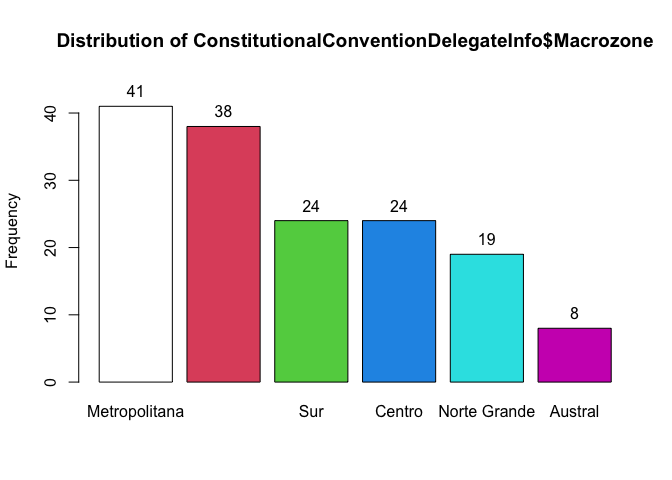
\includegraphics{ChileanCCManuscript_files/figure-latex/figure-3-1.pdf}

Figure 4 displays the variety of professions represented in the
Convention. And this professional diversity yields very similar inputs
as educational diversity. And I argue that this information truly is the
key to unlocking the argument that there was cognitive diversity in the
Convention given the vast array of cognitive processes represented in
the constitution-making body.

Constitution-making is an incredibly complex and technical process.
Technocratic arguments already favor technical expertise over
representation and inclusivity. But these arguments are doubled on
specifically when applied to constitution-making given the intricacies
and legal expertise ``required'' to partake in such processes.
Nonetheless, technical expertise is not always attached or related with
educational experience, which is why either way it is helpful to look at
professions. But Landemore argues that cognitive diversity can and will
make up for lack of technical expertise. Cognitive diversity on its own
is already valuable and conducive to democratic reason, but cognitive
diversity can also make up for technical inexpertise or knowledge on a
subject matter.

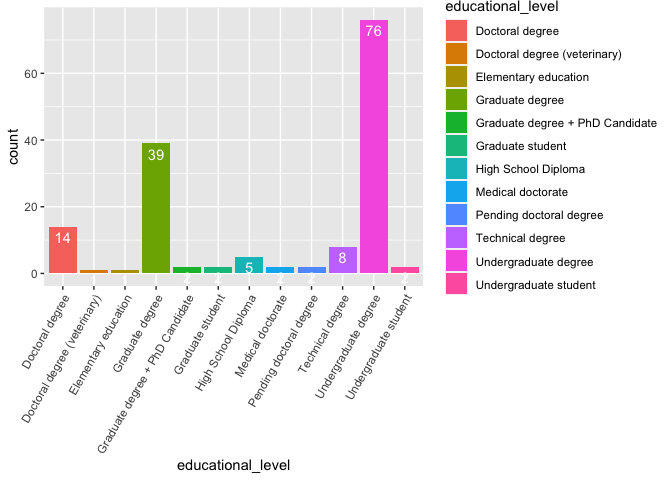
\includegraphics{ChileanCCManuscript_files/figure-latex/figure-4-1.pdf}

Without the procedures that the Chilean Congress designed or imposed
onto the Convention, this degree of representation (and therefore
cognitive diversity) would have not been achieved. Regional
representation would have been achieved given the default on electoral
laws; but it is highly doubtful that the electorate would have been able
to elect a perfectly equal distribution of female and male identifying
delegates. And most definitely, this degree of Indigenous peoples'
representation would have not been possible without these explicit
pieces of legislation that automatically reserved 17 seats out of the
155 seats in the Convention for ten different groups (Chile 2020c).
Furthermore, the facilitated participation of Independents, arguably, is
what most influenced the conditions for there to be cognitive diversity
in the Convention (Chile 2020a). As Independents are people not formally
affiliated with politicians, these are people who have most definitely
not been formally involved in politics. The values and limitations of
this are reviewed at length in my thesis project. But focusing on this
report's aim, by actively involving people that do not have a political
background or profession in a political process, lots of non-political
backgrounds and professions were represented, backgrounds and
professions that require different skill sets, perspectives and
problem-solving abilities.

\hypertarget{party-dynamics}{%
\section{Party Dynamics}\label{party-dynamics}}

This section also considers the impact of the externally imposed
procedure of the participation of Independents on another variable,
party dynamics. The Chilean Congress passed specific laws that first
allowed the participation of Independents in the election of the
Constitutional Convention (Chile 2020a) delegates and then passed
another law that would facilitate their inscription process(Chile
2020b). In other words, Independents were incentivized to participate.
In brief, this was a reflection of the Congress appeasing to the
anti-party mood in Chile after the Social Outbreak protests and the will
of the people to draft a new Constitution by and for ``the people''--
which is why a Constitutional Convention was elected as the
constitution-making organ instead of a Mixed Constitutional Convention
in which half of the body would be made up of elected citizens and half
of current parliamentarians. Chileans, by electing with an overwhelming
electoral majority a Constitution Convention whose all members had to be
elected citizens, demanded to be rid of traditional party-politics for
this process (SERVEL, n.d.).

Figure 5 shows the distribution of the general political parties
represented. I specify that this is the general political party
distribution because most delegates ran under very small Independent
lists and Indigenous peoples groups ran under their particular peoples
groups (Pueblos Originarios). In total and in detail, there technically
were 51 different lists/parties represented among 154 delegates. But
when conflating all of the Independents in one category, and the
Indigenous peoples quotas into on category, we're left with 12
``political parties''-- 10 of these are established Chilean political
parties, one contains all delegates that ran as Independents and one
contains all the different Indigenous delegates representing their
peoples. As Figure 5 shows, Independents overwhelmingly hold the
concentrated majority. A total of 87 of the 154 delegates ran through
Independent lists, and the second largest concentration are the 17
Indigenous peoples' reserved seats. After that, three established
political parties were tied at 10 delegates.

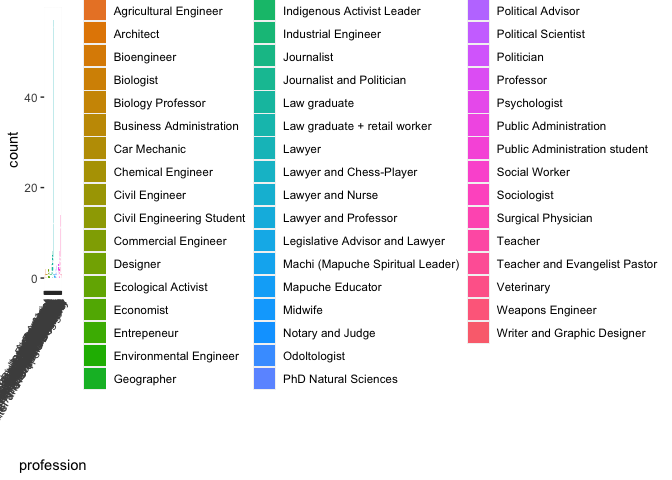
\includegraphics{ChileanCCManuscript_files/figure-latex/figure-5-1.pdf}

Figure 6 shows the distribution of the different political tendencies
represented. Again, I have grouped Independents into a category and
Indigenous peoples into another category. This is to primarily focus on
the distribution of ideologies from the traditional political paries in
Chile. Oficialismo refers to the governing coalition-- considered here
as current-President Gabriel Boric's coalition which encompasses center
to left wing parties. And Oposición refers to the opposing coalition--
considered here as the current opposition of center to right wing
parties. One of the central procedures that my thesis project focuses on
is the 2/3 supermajority voting quorum needed to pass any norm in the
substantive phase of the Process (substantive meaning that what passed,
made it onto the Constitutional Draft). And it is because given that the
opposition (center to right wing parties) were not able to achieve a
third of the seats in the Constitutional Convention, the Chilean right
was left with no bargaining power in agreements as they didn't have an
informal ``veto'' power or the numbers to block motions (Solı́s and Ortiz
2021). As a result, I argue, an entire sector of the Chilean political
spectrum was ignored in negotiations; they did not have to be taken
seriously because they did not have the numbers to be meaningfully
included in negotiations. This, was counterproductive because it
produced an environment of adversarial instead of consensus politics;
delegates from different ideological currents saw each other as barriers
and obstacles to their own goals instead of fellow collaborators, all
because ``what really mattered'' was achieving a 2/3 supermajority
(Solı́s and Ortiz 2021).

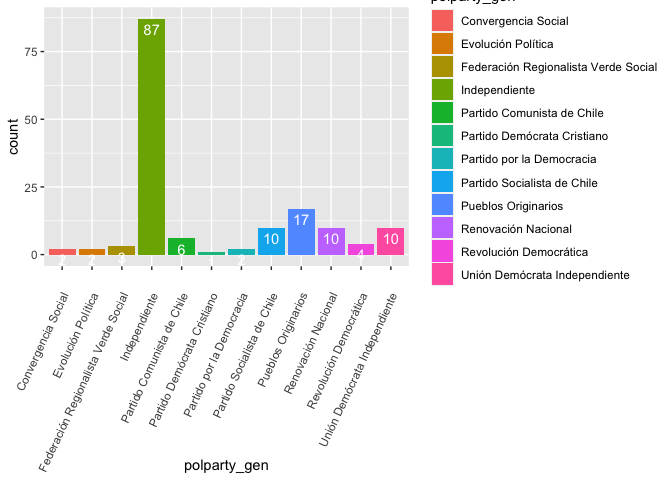
\includegraphics{ChileanCCManuscript_files/figure-latex/figure-6-1.pdf}

\hypertarget{data-analysis-with-regulatory-phase-and-substantive-phase-roll-call-data}{%
\subsection{Data Analysis with Regulatory Phase and Substantive Phase
Roll Call
Data}\label{data-analysis-with-regulatory-phase-and-substantive-phase-roll-call-data}}

Having laid out the general political party and political tendency
distribution, now I will analyze the specific voting behavior of these
different political parties and political tendencies. Figure 7 and 8
show the frequency distribution in the regulatory and substantive phase
of votes casted in favor by members of different political parties.

Figure 7 shows the frequency distribution by political party regarding
the in favor votes casted by the Constitutional Convention delegates in
the Regulatory Phase of the Convention. Visually, the distributions are
relatively similar in the sense that the average for each seem to be
around the 60-70\% of votes casted in favor. Not even getting into
actual statistics, just visuals, I aim to show that political parties in
the regulatory phase acted very similarly. Despite ideological
differences, their voting patterns show there was not much internal
divergences within political parties nor substantial differences
relative to other parties. When drafting the bylaws, political parties
according to their voting behavior, acted similarly internally and
compared to each other.

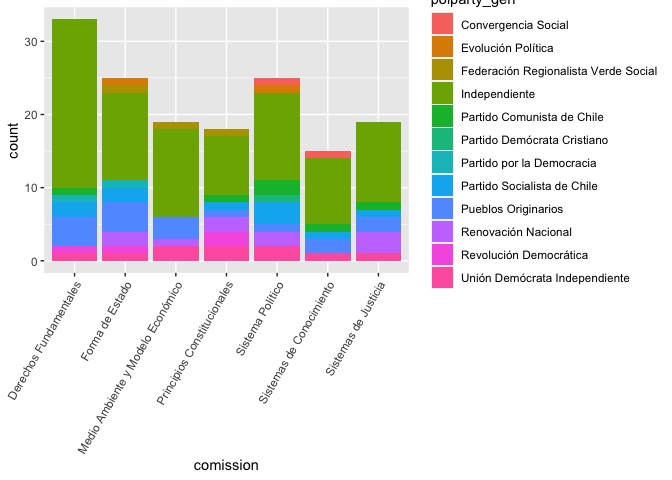
\includegraphics{ChileanCCManuscript_files/figure-latex/figure-7-1.pdf}

But Figure 8, in contrast, shows a completely different voting pattern
and behavior. During the substantive phase, when the votes determined
what kind of content, policies and norms went into the Constitutional
Draft, parties began establishing very distinct behavior to each other.
Independents have the biggest widespread voting frequency, meaning
Independent members voted differently to each other. It makes sense that
they did not demonstrate party unity as they were not an established
party, they were Independents. On the other hand, there is radical
contrast between the party unity of Independents and the party unity of
established parties. Other than that, the Chilean Socialist Party was
the other political grouping that did not display much party unity.
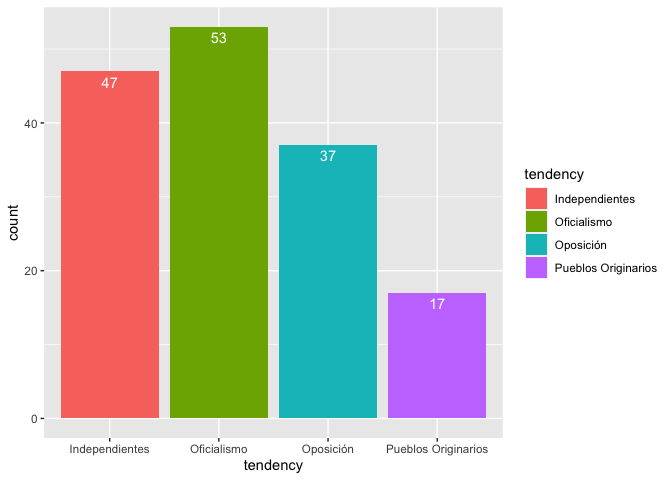
\includegraphics{ChileanCCManuscript_files/figure-latex/figure-8-1.pdf}

Figure 9 and 11 show the frequency distribution in the regulatory and
substantive phase of votes casted in favor by members of different
political tendencies. Boiling down groupings by political trends allows
for a more digestible interpretation for those who aren't familiar with
the Chilean political landscape and spectrum. While it is a
simplification and that can be a limitation, it is a useful way to
process the information. Figure 9 shows that there was not much tendency
unity during the regulatory phase for the debate for the Opposition
coalition and the Indigenous peoples' groups. But that there was
tendency unity for Independents and the Government coalition. While the
Government coalition does have outliars in both extremes, delegates that
voted in favor of a lot of norms and delegates that voted against a lot
of norms, it still displays unity within the political trend.

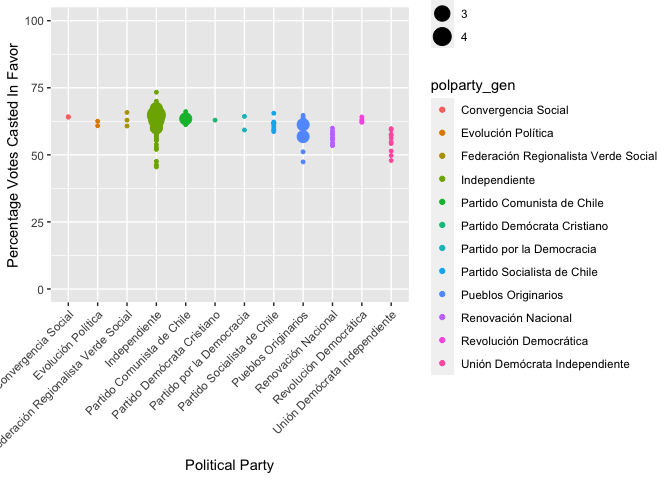
\includegraphics{ChileanCCManuscript_files/figure-latex/figure-9-1.pdf}
Table 10 and Figure 11 show the frequency, distribution and deviation in
the Substantive phase by political tendency. Table 10 numerically shows
via the calculation of standard deviations what is visually displayed in
Figure 11. Table 10 and Figure 11 show that the Independents had the
biggest deviation; which is unsurprising given their whole point was not
to behave like a political party. But surprisingly (or not), the second
largest deviation is the Government's party coalition. The Chilean
center to left parties very publicly became ideologically fragmented,
but this data confirms it numerically and contained in this
constitution-making body. The opposition coalition, the center to right
wing parties displayed a decreased standard deviation by around 35\%,
showing that they remained relatively united throughout the Substantive
phase according to their voting behavior. But the political tendency
with the smallest standard deviation and the narrowest frequency
distribution is the Indigenous peoples' groups. Their voting patterns
remained relatively consistent within that political trend. But also a
potential confounder variable could be that their standard deviation is
lower because they are also the smallest group with only 17 members.
Nonetheless, these voting behaviors show that in the Convention,
Independents and the Government coalition lacked unity within their
political tendency, while the Opposition coalition displayed more unity
but the most united political tendency were the Indigenous peoples'
groups.

\begin{longtable}[]{@{}cc@{}}
\toprule()
Political Tendency & Standard Deviation \\
\midrule()
\endhead
Independientes & 8.54 \\
Oficialismo & 8.30 \\
Oposición & 4.95 \\
Pueblos Originarios & 2.36 \\
\bottomrule()
\end{longtable}

\includegraphics{ChileanCCManuscript_files/figure-latex/figure-11-1.pdf}

\hypertarget{conclusion}{%
\section{Conclusion}\label{conclusion}}

Thus, this report has evaluated the impact of some externally imposed
procedures that aimed to broaden the Constitutional Convention's
inclusivity on the Convention's internal dynamics focusing on cognitive
diversity and party unity. Inclusivity and representation are rightfully
celebrated in democratic processes. Theorists like Landemore, Ho and
Page show how inclusivity and representation can be conducive to
cognitive diversity in a democratic process. They argue that diversity
in a decision-making group is more valuable than the average individual
ability for a group's collective competence particularly in democratic
processes. But the Chilean Constitutional Process seems to be an
outliar. Cognitive diversity was not enough to guarantee the Process'
success and it seemed to hinder the ability of the Convention to reach
meaningful levels of consensus and agreement. While there were high
degrees of representation due to procedural mechanisms that aimed to
purposefully design an inclusive constitution-making organ, and while
there seemed to be cognitive diversity, these features
counter-intuitively hindered democratic reason. They counter-intuitively
hindered democratic reason because they were not conducive to consensus
even after thorough rounds of deliberation and majoritarian votes.
Focusing on these majoritarian votes, it is evident that while the
Convention's parties and political tendencies remained united during the
regulatory phase internally and externally in comparison to other
parties and tendencies, that unity seemed to decrease in the substantive
phase both internally and externally in comparison for other parties and
tendencies.

\hypertarget{references}{%
\section{References}\label{references}}

\hypertarget{refs}{}
\begin{CSLReferences}{1}{0}
\leavevmode\vadjust pre{\hypertarget{ref-cembrano2021propapp}{}}%
Cembrano, Javier, Jose Correa, Gonzalo Diaz, and Victor Verdugo. 2021.
{``Proportional Apportionment: A Case Study from the Chilean
Constitutional Convention.''} In \emph{Equity and Access in Algorithms,
Mechanisms, and Optimization}. EAAMO '21. New York, NY, USA: Association
for Computing Machinery. \url{https://doi.org/10.1145/3465416.3483295}.

\leavevmode\vadjust pre{\hypertarget{ref-ley21216}{}}%
Chile, Congreso de. 2020a. {``Ley 21216.''}
\url{https://www.bcn.cl/leychile/navegar?idNorma=1143661}.

\leavevmode\vadjust pre{\hypertarget{ref-ley21296}{}}%
---------. 2020b. {``Ley 21296.''} 2020.
\url{https://www.bcn.cl/leychile/navegar?idNorma=1153083\&idParte=10182947\&idVersion=2020-12-10}.

\leavevmode\vadjust pre{\hypertarget{ref-ley21298}{}}%
---------. 2020c. {``Ley 21298.''}
\url{https://www.bcn.cl/leychile/navegar?idNorma=1153843}.

\leavevmode\vadjust pre{\hypertarget{ref-servel2022}{}}%
Congreso, Biblioteca Nacional del. n.d. {``Biblioteca Nacional Del
Congreso Plebiscito 2022.''}
\url{https://www.bcn.cl/procesoconstituyente/plebiscito2022}.

\leavevmode\vadjust pre{\hypertarget{ref-elkins2019constitutional}{}}%
Elkins, Zachary, and Alexander Hudson. 2019. {``The Constitutional
Referendum in Historical Perspective.''} In \emph{Comparative
Constitution Making}, 142--64. Edward Elgar Publishing.

\leavevmode\vadjust pre{\hypertarget{ref-delcogdiv}{}}%
Landemore, Hélène. 2012. {``Deliberation, Cognitive Diversity, and
Democratic Inclusiveness: An Epistemic Argument for the Random Selection
of Representatives.''} \emph{Springer}.

\leavevmode\vadjust pre{\hypertarget{ref-landemore2017democratic}{}}%
---------. 2017. \emph{Democratic Reason: Politics, Collective
Intelligence, and the Rule of the Many}. Princeton University Press.

\leavevmode\vadjust pre{\hypertarget{ref-landemore2012collective}{}}%
Landemore, Hélène, and Jon Elster. 2012. \emph{Collective Wisdom:
Principles and Mechanisms}. Cambridge University Press.

\leavevmode\vadjust pre{\hypertarget{ref-servel2020}{}}%
SERVEL. n.d. {``Servicio Electoral de Chile Plebiscito 2020.''}
\url{https://historico.servel.cl/servel/app/index.php?r=EleccionesGenerico\&id=10}.

\leavevmode\vadjust pre{\hypertarget{ref-interferencia1}{}}%
Solı́s, Camilo, and Diego Ortiz. 2021. {``¿Caduc{ó} Acuerdo Del 15 de
Noviembre?''}
\url{https://interferencia.cl/articulos/caduco-acuerdo-del-15-de-noviembre-derecha-no-logra-13-de-constituyente-e-izquierda-e}.

\end{CSLReferences}

\end{document}
